%% notes-tex/multimodal/043-datasets-primer/sections/3-agreement.tex

\section{Agreement within and between datasets\secstatus{todo}}
\label{sec:agreement}

\subsection{Within a dataset\secstatus{todo}}
\label{sec:within}

A dataset's agreement with itself bounds both what a model can score on it and what
any other dataset can agree with it. The new measurements are in
\file{experiments/043-expression-proteome-morphology/scripts/within_dataset_ceilings.py}
(slurm jobs 5893 for Kemmeren and Hu, 5895, 5896 and 5898 for Jackson, the segregants and the figures).

\notesec{Jackson 2020}
Each of the 784 records is one construction in one condition, a median of 23
cells and 43{,}851 UMIs (IQR 19{,}757 to 101{,}152); YPD and rapamycin reach a median of about 400{,}000
UMIs per construction, the other nine conditions 14{,}000 to 93{,}000. Within one condition, two constructions of the same
genotype agree on their deletion-effect profiles only slightly better than two
constructions of different genotypes (Table~\ref{tab:jackson},
Fig.~\ref{fig:ceilings}a): a median $r$ of 0.129 against 0.095 with every gene of at
least 100 UMIs in the condition (1{,}778 same-genotype and 21{,}300 different-genotype
pairs). The gap widens on the 660 deepest genes (0.244 against 0.103 at 1{,}000 UMIs)
and when only genes covered in both constructions are kept, but that second rule scores
fewer pairs, the deep ones. The different-genotype pairs are not near zero because both
constructions are divided by the same HO reference. The Jackson ceiling for one
construction's deletion effect is therefore low; most of a record's deviation from HO is
count noise shared with any other construction in the flask.

%% SOURCE: experiments/043-expression-proteome-morphology/scripts/primer_043_tables.py
%% -> tables/t4-jackson.tex
\begin{table}[htbp]
\centering
\scriptsize
\setlength{\tabcolsep}{3pt}
\caption[]{\textbf{Jackson 2020, construction against construction within one
condition.} Pooled over the 11 conditions. Level profile: Pearson over genes of
$\log_2(\mathrm{CPM}+1)$; deletion effect: of $\log_2((\mathrm{CPM}+1)/
(\mathrm{CPM}_{\mathrm{HO}}+1))$ against the six HO constructions summed, HO pairs left
out. A gene enters every pair of a condition when its UMIs summed over that condition
reach the floor. Same genotype: two of the six constructions of one genotype; different:
two constructions of different genotypes in the same flask.}
\label{tab:jackson}
%% GENERATED by experiments/043-expression-proteome-morphology/scripts/primer_043_tables.py
%% SOURCE: results/store_census.json, results/cross_dataset_correlation.json,
%% results/within_dataset_ceilings.json and the 019 ceiling files named in
%% tables/provenance.json. Do not edit by hand.

\begin{tabular}{>{\raggedright\arraybackslash}p{50mm}>{\raggedleft\arraybackslash}p{30mm}>{\raggedleft\arraybackslash}p{30mm}>{\raggedleft\arraybackslash}p{24mm}>{\raggedleft\arraybackslash}p{20mm}}
\toprule
Gene rule & Level profile r, median, same vs different genotype & Deletion-effect r, median, same vs different genotype & Pairs, n, same / different & Genes per pair, median \\
\midrule
$\geq$ 10 UMIs summed over the condition & 0.637 vs 0.620 & 0.184 vs 0.157 & 1{,}778 / 21{,}300 & 5{,}405 \\
$\geq$ 100 UMIs summed over the condition & 0.654 vs 0.612 & 0.129 vs 0.095 & 1{,}778 / 21{,}300 & 3{,}701 \\
$\geq$ 1000 UMIs summed over the condition & 0.919 vs 0.887 & 0.244 vs 0.103 & 1{,}778 / 21{,}300 & 660 \\
$\geq$ 10 UMIs in both constructions & 0.941 vs 0.925 & 0.406 vs 0.244 & 1{,}742 / 20{,}866 & 490 \\
$\geq$ 100 UMIs in both constructions & 0.968 vs 0.951 & 0.414 vs 0.164 & 1{,}191 / 12{,}337 & 34 \\
$\geq$ 1000 UMIs in both constructions & 0.997 vs 0.991 & 0.600 vs 0.112 & 271 / 2{,}924 & 0 \\
\bottomrule
\end{tabular}

\end{table}

\notesec{Kemmeren 2014}
GEO titles name the culture: \texttt{bck1-del-1-a} and \texttt{-1-b} are the
dye-swapped arrays of culture 1. Of 1{,}480 mutants whose titles parse, 114 carry two
cultures, 72 in the responsive series GSE42527 and 42 in the non-responsive series
GSE42526; the other 1{,}366 have one (16 arrays with irregular titles are left out).
Culture 1 against culture 2 of the same mutant gives a median per-strain $r$ of 0.730,
against 0.284 for culture 1 of one mutant and culture 2 of another
(Table~\ref{tab:kemmeren}, Fig.~\ref{fig:ceilings}b). Across the 114 mutants the median
per-gene $r$ is 0.612, so the own-culture ceiling is 0.729 by test-retest and 0.653 by
decomposition (Fig.~\ref{fig:ceilings}c). The two differ because the 114 paired mutants
are enriched for strong responders, while the decomposition takes its signal variance
from all 1{,}480. These numbers replace the void 0.775. The stored record averages both
cultures where two exist; hypothesis, untested, that its ceiling is higher than the
single-culture one.

%% SOURCE: experiments/043-expression-proteome-morphology/scripts/primer_043_tables.py
%% -> tables/t5-kemmeren.tex
\begin{table}[htbp]
\centering
\footnotesize
\caption[]{\textbf{Kemmeren 2014, culture 1 against culture 2.} A culture's profile is the
mean over its dye-swapped arrays of the within-array $\log_2$(deletion/reference pool),
computed by the loader's own functions from the GEO arrays of GSE42527 and GSE42526. The
null pairs culture 1 of one mutant with culture 2 of another. Per-gene ceilings average
over genes with at least three paired mutants; the decomposition takes the noise variance
from the paired cultures and the total variance from the first culture of every mutant.}
\label{tab:kemmeren}
%% GENERATED by experiments/043-expression-proteome-morphology/scripts/primer_043_tables.py
%% SOURCE: results/store_census.json, results/cross_dataset_correlation.json,
%% results/within_dataset_ceilings.json and the 019 ceiling files named in
%% tables/provenance.json. Do not edit by hand.

\begin{tabular}{>{\raggedright\arraybackslash}p{95mm}>{\raggedleft\arraybackslash}p{50mm}}
\toprule
Kemmeren 2014 own-culture statistic & Value \\
\midrule
Mutants with two cultures, n (responsive / non-responsive series) & 114 of 1{,}480 (72 / 42) \\
Per-strain r across genes, median [IQR] & 0.730 [0.602, 0.835] \\
Per-strain r, different mutants (null), median & 0.284 \\
Per-gene r across mutants, median [IQR] & 0.612 [0.431, 0.754] (6{,}169 genes) \\
Ceiling, test-retest: mean over genes of $\sqrt{r_g}$ & 0.729 \\
Ceiling, decomposition: mean over genes of $\sqrt{1 - \sigma^2_{e,g}/\sigma^2_g}$ & 0.653 \\
Void 019 cross-study ceiling (Sameith pair, identical arrays) & 0.775 \\
\bottomrule
\end{tabular}

\end{table}

\notesec{Hu 2007}
No replicate statistic is computable. The paper says ``Each experiment was
independently carried out at least twice'' (paper.md line 55), and the replicates were
combined before release: the group ``performed weighted duplicate averaging with custom
Java software'' (line 59). GEO GSE4654 holds one X score per strain; the per-array data
went to the Longhorn Array Database and a lab site that was never archived. The only
available bound is the agreement with Kemmeren, a median per-genotype $r$ of 0.107 over
255 deletions and a per-gene $r$ of 0.097 (Table~\ref{tab:cross}). That agreement is a floor on Hu's reproducible signal;
no ceiling is measured.

\notesec{Boocock 2025 and N'Guessan 2025}
Neither panel has a replicate: every pooled record sums the cells of one
segregant (a median of 17 for Boocock Ap, 3 for N'Guessan), and the per-cell counts are
not stored, so no split-half is possible (Table~\ref{tab:segregants}). No segregant
appears in two panels: on a 5 kb grid of called parents the best concordance of any of
the 393 pooled segregants with any of 27{,}744 de novo BY $\times$ RM cells is a median
of 0.672, and with any of the 2{,}951 N'Guessan segregants 0.657, where unrelated
segregants share half the genome and identity would be near 1; none reaches 0.95
(Fig.~\ref{fig:segregants}b). A weaker test still asks whether genotype carries
expression across panels. For each pooled segregant, the 20 de novo cells nearest in
genotype (mean concordance 0.647) agree with its deviation from the panel mean at a
median $r$ of 0.113, against 0.070 for 20 random cells; the paired difference is 0.040
(388 segregants, 63\% positive, Wilcoxon $p = 1\times10^{-8}$). The single nearest
N'Guessan segregant gives 0.101 against 0.060 (381 segregants, $p = 0.009$). At the panel
level the summed BY $\times$ RM profiles agree at $r$ = 0.872 between Boocock's pooled
and de novo panels and 0.693 between Boocock's pooled panel and N'Guessan, which grew in
YPD rather than minimal medium. Genotype posteriors differ by panel: a median 0\% of
markers of a pooled Boocock segregant and 1.7\% of an N'Guessan one are called with
posterior below 0.9, against 24 to 35\% for a de novo cell.

%% SOURCE: experiments/043-expression-proteome-morphology/scripts/primer_043_tables.py
%% -> tables/t6-segregants.tex
\begin{table}[htbp]
\centering
\scriptsize
\setlength{\tabcolsep}{3pt}
\caption[]{\textbf{The segregant panels.} A pooled record sums the cells matched to one
previously genotyped segregant; a de novo record is one cell genotyped from its own
transcripts. The posterior column is the
marker-weighted fraction of a genotype whose called parent has posterior below 0.9.}
\label{tab:segregants}
%% GENERATED by experiments/043-expression-proteome-morphology/scripts/primer_043_tables.py
%% SOURCE: results/store_census.json, results/cross_dataset_correlation.json,
%% results/within_dataset_ceilings.json and the 019 ceiling files named in
%% tables/provenance.json. Do not edit by hand.

\begin{tabular}{>{\raggedright\arraybackslash}p{40mm}>{\raggedleft\arraybackslash}p{18mm}>{\raggedleft\arraybackslash}p{18mm}>{\raggedleft\arraybackslash}p{18mm}>{\raggedleft\arraybackslash}p{18mm}>{\raggedleft\arraybackslash}p{18mm}>{\raggedleft\arraybackslash}p{18mm}}
\toprule
Panel & Records, n & Cells, n & Cells per record, median & UMIs per record, median & Genes detected per record, median & Marker fraction with posterior $<$ 0.9, median \\
\midrule
Boocock Ap, pooled BY $\times$ RM & 393 & 7{,}124 & 17 & 27{,}902 & 3{,}595 & 0.000 \\
Boocock A, de novo BY $\times$ RM & 27{,}744 & 27{,}744 & 1 & 4{,}017 & 1{,}228 & 0.236 \\
Boocock B, de novo YJM145 $\times$ YPS163 & 44{,}784 & 44{,}784 & 1 & 2{,}130 & 859 & 0.352 \\
Boocock 3004, de novo CBS2888 $\times$ YJM981 & 6{,}595 & 6{,}595 & 1 & 1{,}982 & 605 & 0.297 \\
N'Guessan, pooled BY $\times$ RM & 2{,}951 & 14{,}263 & 3 & 18{,}221 & 2{,}592 & 0.017 \\
\bottomrule
\end{tabular}

\end{table}

%% SOURCE: experiments/043-expression-proteome-morphology/scripts/within_dataset_ceilings.py
%% -> figures/within_dataset_ceilings_2026-10-19-16-49-03.pdf and figures/within_dataset_segregants_2026-10-19-16-49-04.pdf
\begin{figure}[htbp]\centering
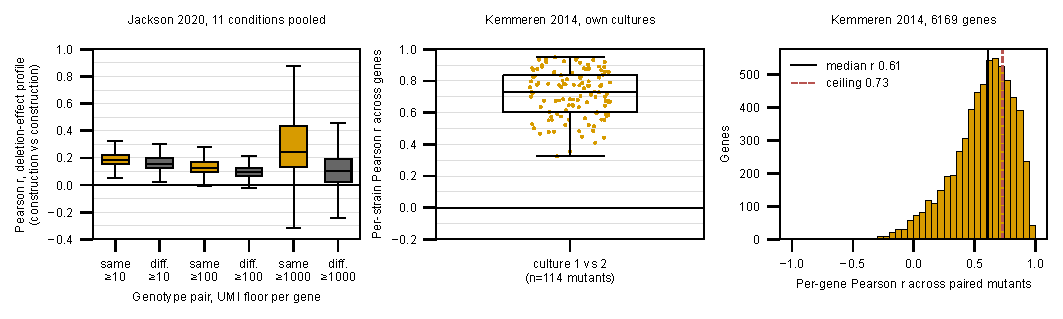
\includegraphics[width=\textwidth]{figures/within_dataset_ceilings_2026-10-19-16-49-03.pdf}\par\vspace{2pt}
\caption[]{\textbf{Two datasets measured against themselves.} \textbf{a}, Jackson 2020:
Pearson over genes of the deletion-effect profiles of two constructions in one condition,
same genotype (orange) against different genotypes (gray), at three floors on a gene's
UMIs summed over the condition; 1{,}778 and 21{,}300 pairs per floor, 11 conditions
pooled, HO pairs left out. \textbf{b}, Kemmeren 2014: Pearson across genes between the two
cultures of each of the 114 mutants profiled twice; culture 1 of one mutant against
culture 2 of another gives a median of 0.284 (not drawn). \textbf{c}, per-gene Pearson
across the 114 mutants for 6{,}169 genes, with the median $r$ and the ceiling, the mean
over genes of $\sqrt{\max(r_g, 0)}$.}
\label{fig:ceilings}
\end{figure}
%% Generated by experiments/043-expression-proteome-morphology/scripts/within_dataset_ceilings.py

\begin{figure}[htbp]\centering
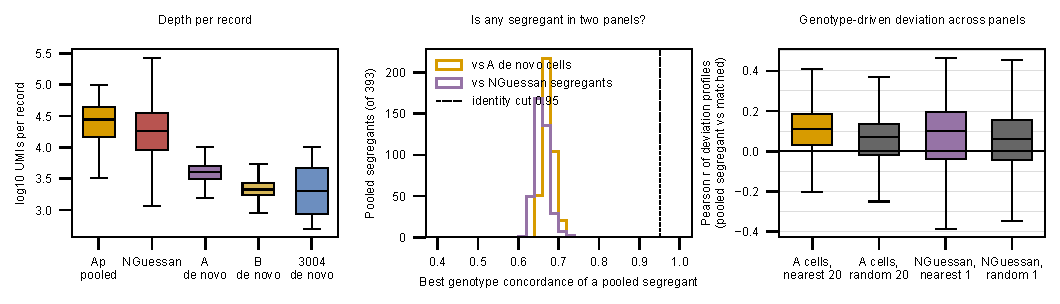
\includegraphics[width=\textwidth]{figures/within_dataset_segregants_2026-10-19-16-49-04.pdf}\par\vspace{2pt}
\caption[]{\textbf{The segregant panels have no shared segregant and a weak shared
genotype signal.} \textbf{a}, UMIs per record by panel (pooled records sum a segregant's
cells, de novo records are single cells). \textbf{b}, for each of the 393 pooled Boocock
segregants, the best genotype concordance with any de novo cross-A cell (orange) or any
N'Guessan segregant (purple), on a 5 kb grid of called parents; the dashed line marks
0.95. \textbf{c}, Pearson over genes between a pooled segregant's deviation from its
panel and that of its 20 nearest de novo cells, 20 random cells, its nearest N'Guessan
segregant, or a random one; genes with at least 10 UMIs on both sides.}
\label{fig:segregants}
\end{figure}
%% Generated by experiments/043-expression-proteome-morphology/scripts/within_dataset_ceilings.py

\subsection{Between datasets\secstatus{todo}}
\label{sec:between}

Records are matched by perturbed gene names and environment (isolates by strain name),
and each pair is scored per shared genotype, across shared genes, and per shared gene,
across shared genotypes (Table~\ref{tab:cross}, Fig.~\ref{fig:pergenotype};
\file{experiments/043-expression-proteome-morphology/scripts/cross_dataset_correlation.py},
slurm jobs 5890 and 5892). Every pair compares log against log, so the base of a
logarithm does not change a correlation.

%% SOURCE: experiments/043-expression-proteome-morphology/scripts/primer_043_tables.py
%% -> tables/t7-cross.tex
\begin{table}[htbp]
\centering
\scriptsize
\setlength{\tabcolsep}{3pt}
\caption[]{\textbf{Agreement between datasets of the same readout type.} Per genotype:
Pearson and Spearman across the shared genes (at least 20). Per gene: Pearson across the
shared genotypes (at least 5). Jackson is turned into a deletion effect against HO in the
same environment; Messner and Zelezniak are log ratios to their record reference; Caudal
and Muenzner are centered per gene over the isolates. The Jackson environment row pairs
one genotype across two environments (605 genotype-environment pairs).}
\label{tab:cross}
%% GENERATED by experiments/043-expression-proteome-morphology/scripts/primer_043_tables.py
%% SOURCE: results/store_census.json, results/cross_dataset_correlation.json,
%% results/within_dataset_ceilings.json and the 019 ceiling files named in
%% tables/provenance.json. Do not edit by hand.

\begin{tabular}{>{\raggedright\arraybackslash}p{46mm}>{\raggedleft\arraybackslash}p{16mm}>{\raggedleft\arraybackslash}p{30mm}>{\raggedleft\arraybackslash}p{18mm}>{\raggedleft\arraybackslash}p{26mm}>{\raggedleft\arraybackslash}p{20mm}}
\toprule
Pair & Shared genotypes, n & Per-genotype Pearson r, median [IQR] & Per-genotype Spearman, median & Per-gene Pearson r, median (genes, n) & Genes with per-gene r $>$ 0.3, fraction \\
\midrule
Kemmeren $\times$ Sameith Sm & 82 & 1.000 [1.000, 1.000] & 1.000 & 1.000 (6{,}169) & 1.000 \\
Kemmeren $\times$ Hu & 255 & 0.107 [0.013, 0.184] & 0.082 & 0.097 (5{,}803) & 0.102 \\
Kemmeren $\times$ Nadal, YPD & 913 & 0.002 [$-$0.017, 0.022] & 0.007 & 0.017 (5{,}891) & 0.007 \\
Kemmeren $\times$ Nadal, NaCl & 920 & $-$0.001 [$-$0.021, 0.022] & 0.005 & 0.015 (5{,}896) & 0.006 \\
Kemmeren $\times$ Jackson, YPD 10 h & 11 & 0.043 [0.026, 0.070] & 0.047 & 0.035 (5{,}340) & 0.247 \\
Kemmeren $\times$ Jackson, YPD 4 h (a) & 11 & 0.066 [0.027, 0.210] & 0.030 & 0.118 (5{,}353) & 0.321 \\
Kemmeren $\times$ Jackson, YPD 4 h (b) & 11 & 0.076 [0.036, 0.149] & 0.045 & 0.052 (5{,}601) & 0.253 \\
Nadal YPD $\times$ Nadal NaCl & 2{,}952 & 0.208 [0.168, 0.231] & 0.043 & 0.183 (6{,}134) & 0.050 \\
Nadal duplicates, one condition & 105 & 0.376 [0.323, 0.452] & 0.178 & 0.062 (5{,}897) & 0.089 \\
Jackson, environment $\times$ environment & 605 & 0.010 [$-$0.005, 0.029] & 0.009 & n/a & n/a \\
Messner $\times$ Zelezniak (protein) & 89 & 0.049 [$-$0.016, 0.185] & 0.050 & 0.085 (715) & 0.067 \\
Kemmeren mRNA $\times$ Messner protein & 1{,}349 & 0.031 [$-$0.025, 0.112] & 0.034 & 0.094 (1{,}832) & 0.033 \\
Caudal mRNA $\times$ Muenzner protein & 759 & 0.208 [0.109, 0.307] & 0.176 & 0.160 (1{,}572) & 0.183 \\
Muenzner turnover $\times$ abundance & 55 & $-$0.006 [$-$0.053, 0.047] & $-$0.003 & $-$0.007 (1{,}120) & 0.066 \\
\bottomrule
\end{tabular}

\end{table}

\notesec{Sameith 2015 single mutants are Kemmeren 2014's arrays}
All 82 Sameith Sm profiles are value-for-value identical to Kemmeren's for the same
deletions (median per-genotype $r$ = 1.000), and the GEO deposits show why. GSE42536
holds 144 Sameith single-mutant arrays: 115 are byte-identical re-deposits of GSE42527 or
GSE42526 arrays, and the other 29 match a Kemmeren array exactly on the normalized Cy5
and Cy3 signal columns. Sameith's Methods defer to the earlier paper: ``Full details of
all gene expression profiling procedures have been described before [46]''. The pair is
therefore no replicate, and the experiment 019 expression ceiling built on it
(test-retest 0.744 per strain, ceiling 0.77) is void; Table~\ref{tab:kemmeren} replaces
it. The 143 Sameith double-mutant arrays are new hybridizations.

\notesec{Nadal-Ribelles 2025}
Nadal-Ribelles agrees with Kemmeren at a median per-genotype $r$ of 0.002 in YPD (913
deletions) and with itself not much better. Experiment 028 measured the same genotype
across batches at a median $r$ of 0.043 against 0.022 for different genotypes, and
split halves at 0.080 against 0.051. The 0.376 of within-condition duplicates in
Table~\ref{tab:cross} is Pearson driven by a few extreme log fold changes (the Spearman
of the same pairs is 0.178); hypothesis, untested, that they come from genes with
near-zero counts on one side.

\notesec{Jackson 2020 across environments}
One TF deletion's effect profile in one environment agrees with the same deletion's
profile in another at a median $r$ of 0.010 (605 pairs). The paper reports that TF
deletions change far fewer genes than conditions do (96 differentially expressed genes in
YPD, 160 in rapamycin), so a near-zero cross-environment agreement is what the paper
leads one to expect; it does not show the data to be noise, and the within-condition
construction pairs above measure the noise directly.

\notesec{mRNA against protein}
Deletions agree weakly: Kemmeren against Messner gives a median per-genotype $r$ of 0.031
over 1{,}349 deletions and a per-gene $r$ of 0.094 over 1{,}832 genes. Isolates agree
more: Caudal against Muenzner gives 0.208 over 759 isolates and 0.160 per gene. Protein
varies far more across isolates than across deletions (Fig.~\ref{fig:mrnaprot}, left, x axes); hypothesis, untested, that this larger range is why the two readouts agree more
there. Turnover against abundance is near zero (55 isolates).

\notesec{Expression to morphology}
A ridge from each gene-level matrix to the 281 CalMorph features of the shared Ohya
genotypes (5-fold out-of-fold, one row-permutation null) is the one cross-label link that
matters for a held-out probe (Table~\ref{tab:morph}, Fig.~\ref{fig:mrnaprot}, right). Kemmeren
carries the most signal per genotype; Messner reaches nearly as far on three times the
genotypes.

%% SOURCE: experiments/043-expression-proteome-morphology/scripts/primer_043_tables.py
%% -> tables/t8-morphology.tex
\begin{table}[htbp]
\centering
\footnotesize
\caption[]{\textbf{Ridge from a gene-level matrix to CalMorph.} Out-of-fold Pearson per
CalMorph feature across held-out genotypes; inputs and targets z-scored and clipped at 8,
penalty chosen on an inner split. The 116 moving features are the experiment 019 list
(\file{calmorph_moving_features.json} on the multimodal-phenotype-retrospective
worktree).}
\label{tab:morph}
%% GENERATED by experiments/043-expression-proteome-morphology/scripts/primer_043_tables.py
%% SOURCE: results/store_census.json, results/cross_dataset_correlation.json,
%% results/within_dataset_ceilings.json and the 019 ceiling files named in
%% tables/provenance.json. Do not edit by hand.

\begin{tabular}{>{\raggedright\arraybackslash}p{30mm}>{\raggedleft\arraybackslash}p{26mm}>{\raggedleft\arraybackslash}p{26mm}>{\raggedleft\arraybackslash}p{26mm}>{\raggedleft\arraybackslash}p{26mm}}
\toprule
Input matrix & Genotypes shared with Ohya, n & Mean r over 281 features & Row-permutation null, mean r & Median r over 116 moving features \\
\midrule
Kemmeren 2014 & 1{,}437 & 0.238 & $-$0.005 & 0.348 \\
Messner 2023 & 4{,}279 & 0.179 & 0.008 & 0.278 \\
Hu 2007 & 259 & 0.114 & $-$0.052 & 0.235 \\
Sameith 2015 Sm & 81 & $-$0.014 & $-$0.077 & $-$0.085 \\
\bottomrule
\end{tabular}

\end{table}

%% SOURCE: experiments/043-expression-proteome-morphology/scripts/cross_dataset_correlation.py
%% -> figures/cross_dataset_per_genotype_pearson_2026-10-19-14-37-41.pdf, figures/cross_dataset_mrna_protein_per_gene_2026-10-19-14-37-41.pdf, figures/cross_dataset_morphology_ridge_2026-10-19-14-37-41.pdf
\begin{figure}[htbp]\centering
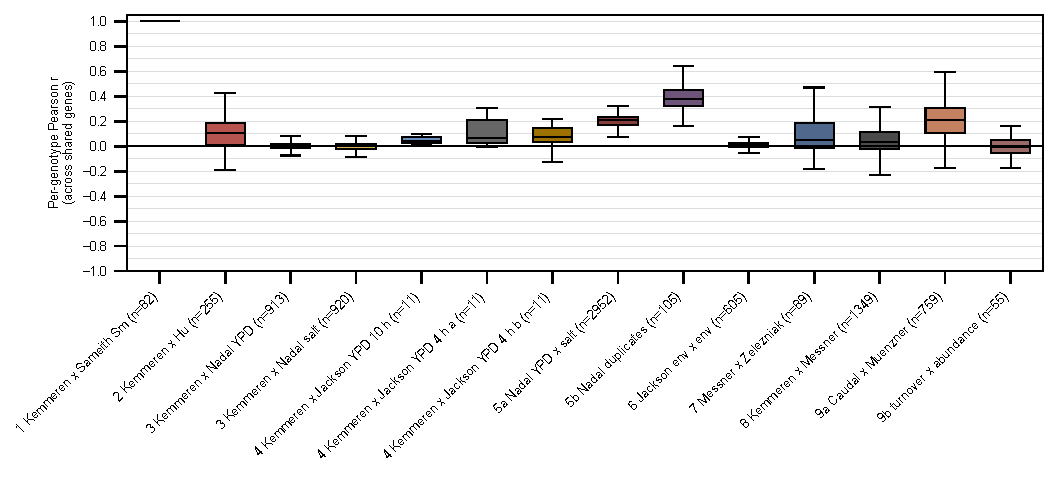
\includegraphics[width=\textwidth]{figures/cross_dataset_per_genotype_pearson_2026-10-19-14-37-41.pdf}\par\vspace{2pt}
\caption[]{\textbf{Agreement between datasets is low except for the Sameith copy.} Per
shared genotype, Pearson across the shared genes for every pair of Table~\ref{tab:cross};
boxes are quartiles, whiskers 1.5 IQR, outliers not drawn.}
\label{fig:pergenotype}
\end{figure}
%% Generated by experiments/043-expression-proteome-morphology/scripts/cross_dataset_correlation.py

\begin{figure}[htbp]\centering
\begin{minipage}[b]{0.49\textwidth}\centering
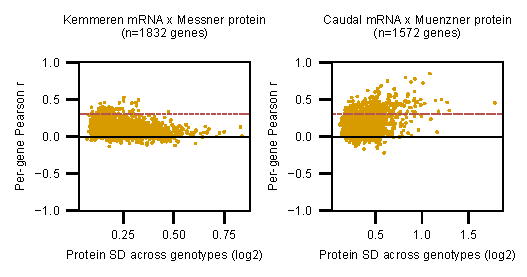
\includegraphics[width=\linewidth]{figures/cross_dataset_mrna_protein_per_gene_2026-10-19-14-37-41.pdf}
\end{minipage}\hfill
\begin{minipage}[b]{0.49\textwidth}\centering
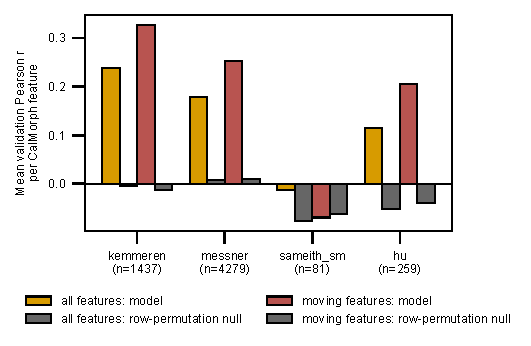
\includegraphics[width=\linewidth]{figures/cross_dataset_morphology_ridge_2026-10-19-14-37-41.pdf}
\end{minipage}\par\vspace{2pt}
\caption[]{\textbf{mRNA against protein, and expression to morphology.} Left two panels:
per-gene Pearson between mRNA and protein across the shared genotypes, against the
protein's SD across those genotypes, for 1{,}832 genes over the deletions of Kemmeren and
Messner and 1{,}572 genes over the isolates of Caudal and Muenzner; the dashed line marks
$r$ = 0.3. Right: mean out-of-fold Pearson per CalMorph feature of a ridge from each input
matrix (Table~\ref{tab:morph}), with its row-permutation null.}
\label{fig:mrnaprot}
\end{figure}
%% Generated by experiments/043-expression-proteome-morphology/scripts/cross_dataset_correlation.py
